\documentclass{beamer}

%% Math
\usepackage{amsmath}
\usepackage{amsfonts}
\usepackage{amssymb}
\usepackage{amsthm}
% \usepackage{lmodern}
\usepackage{eucal}
\usepackage{carlos-variables}
\usepackage{mleftright}
\mleftright

\usepackage[T2A,T1]{fontenc}
\usepackage[utf8]{inputenc}


%% Mis
\usepackage{graphicx}
\graphicspath{{figures/}}

\usepackage{microtype}
\usepackage[inline]{enumitem}

%% Beamer options
\usetheme{Boadilla}
\usecolortheme{default}
\usefonttheme{professionalfonts}

\begin{document}
%% Title
\title{Tropicalization of Character Varieties}%
\author[TGG]{Tropical Geometry Group}%
\subject{character varieties, tropical geometry}%

\frame{\titlepage}%

%% Frames
\begin{frame}
  \frametitle{Visualizing Tropical Character Varieties}
  \framesubtitle{Part I}%
  Summary of work: Our group worked on visualization of tropicalized
  character varieties into $\SL_2\bbC$ of $\bbZ\times\bbZ$ and $\bbZ*\bbZ$
  as well as several knot groups whose $A$-polynomials we obtained from a
  paper by Eric Chesebro \emph{Formulas for Character Varieties of
    $2$-Bridge Knots} which can be found on his website
  \url{http://hs.umt.edu/math/research/technical-reports/documents/2012/KnotFormulas.pdf}.

  With the help of \texttt{Mathematica}, we made the following subdivision
  of the Newton polytopes of these character varieties.
\end{frame}

\begin{frame}
  \frametitle{Visualizing Tropical Character Varieties}
  \framesubtitle{Part II}
  Some pictures
  \begin{figure}
    
\includegraphics[scale=0.5]{newtonsub_apoly_fig8}
    \caption{Subdivided Newton polytope for the $A$-polynomial of the
      figure-$8$ knot.}
  \end{figure}
\end{frame}
\begin{frame}
  \begin{figure}
    
\includegraphics[scale=0.45]{newtonsub_apoly_twist4}
    \caption{Subdivided Newton polytope for the $A$-polynomial the
      $4$-twisted knot.}
  \end{figure}
\end{frame}

\begin{frame}
  \frametitle{Visualizing Tropical Character Varieties}
  \framesubtitle{Part III} Some more pictures for Newton polytopes of two
  $2$-bridge knots corresponding to $\varphi(1)$ and $\varphi(2)$ of
  Chesebro's equation.
  \[
    
\includegraphics[scale=0.5]{newtonsub_phi1}
    \quad
    
\includegraphics[scale=0.5]{newtonsub_phi2}
  \]
\end{frame}

%%% Local Variables:
%%% mode: latex
%%% TeX-master: "../MRC16-Trop-CharVars-Slides"
%%% End:
%
\begin{frame}{$S_{2,g}$ - a recursive approach}

  \begin{definition}
    $S_{2,g}$ is the number of words over an alphabet of size $g$ such
    that no letter appears (considering absolute multiplicities) more
    than twice.
  \end{definition}

  \pause

  \begin{definition}
    $S_{2,g}^{d,l,u}$ is the number of words counted by $S_{2,g}$ which
    have exactly $d$ exponents of $\pm 2$, have \emph{reduced} length
    $l$ (exponents are ignored), and use exactly $u$ distinct letters.
  \end{definition}

  \pause

  \[S_{2,g} = \sum_{d=0}^{g} \sum_{l=0}^{2g} \sum_{u=0}^{g}
    S_{2,g}^{d,l,u}, \]
  and
  \[ S_{2,0}^{0,0,0} = 1. \]


\end{frame}

\begin{frame}{The recursion}

  {\tiny
    \begin{align*}
      S_{2,g}^{d,l,u} =& S_{2,g-1}^{d,l,u} \\
                       &+\sum_{j=0}^{u-1} {g-1 \choose j} \cdot j! \cdot 2^j \cdot (l - 2j) \cdot \left( S_{2,g-1-j}^{d, l-1-2j, u-j-1} + S_{2,g-1-j}^{d-1,l-1-2j,u-j-1} \right) \cdot 2 \\
                       &+  \sum_{j=0}^{u-1} \sum_{k=0}^{u-1-j} { g-1 \choose j + k} \cdot (j + k)! \cdot 2^{j + k} \cdot \frac{(l - 2(j + k) - 1) \cdot (l - 2 (j + k) - 2)}{2} \cdot S_{2,g-1-j-k}^{d,l-2(j+k) - 2,u-1-j-k} \cdot 4 \\
                       &+ \sum_{j=0}^{0} \sum_{k=1}^{u-1-j} { g-1 \choose j + k} \cdot (j + k)! \cdot 2^{j + k} \cdot \frac{(l - 2(j + k) - 1) \cdot 2}{2} \cdot S_{2,g-1-j-k}^{d,l-2(j+k) - 2,u-1-j-k} \cdot 4 \\
                       &+ \sum_{j=1}^{u-1} \sum_{k=0}^{0} { g-1 \choose j + k} \cdot (j + k)! \cdot 2^{j + k} \cdot \frac{(l - 2(j + k) - 1) \cdot 2}{2} \cdot S_{2,g-1-j-k}^{d,l-2(j+k) - 2,u-1-j-k} \cdot 4 \\
                       &- \sum_{j=1}^{u-1} \sum_{k=1}^{u-1-j} { g-1 \choose j + k} \cdot (j + k)! \cdot 2^{j + k} \cdot \frac{(l - 2(j + k) - 1) \cdot 2}{2} \cdot S_{2,g-1-j-k}^{d,l-2(j+k) - 2,u-1-j-k} \cdot 4 \\
                       &+ \sum_{j=1}^{u-1} \sum_{k=0}^{u-1-j} { g-1 \choose j + k} \cdot (j + k)! \cdot 2^{j + k} \cdot \frac{(l - 2(j + k) - 1) \cdot 2(j-1)}{2} \cdot S_{2,g-1-j-k}^{d,l-2(j+k) - 2,u-1-j-k} \cdot 4\\
                       &+ \sum_{j=1}^{u-1} \sum_{k=1}^{u-1-j} { g-1 \choose j + k} \cdot (j + k)! \cdot 2^{j + k} \cdot \frac{(l - 2(j + k) - 1) \cdot 2)}{2} \cdot S_{2,g-1-j-k}^{d,l-2(j+k) - 2,u-1-j-k} \cdot 4\\
    \end{align*}
  }

\end{frame}

\begin{frame}{Some calculations}
  This has been implemented, with the following results
  \begin{align*}
    S_{2,0} &= 1 \\
    S_{2,1} &= 5 \\
    S_{2,2} &= 105 \\
    S_{2,3} &= 6061 \\
    S_{2,4} &= 668753 \\
    &\vdots
  \end{align*}

  Conclusion: it is impractical to consider naïve generators when examining
  representations $F_n$ to $\SL_2\bbC$.
\end{frame}

%%% Local Variables:
%%% mode: latex
%%% TeX-master: "../MRC16-Trop-CharVars-Slides"
%%% End:
%
\begin{frame}
  \frametitle{Tropicalization of $\frakX(F_3,\SL_2\bbC)$}
  The character variety $\frakX(F_3, \SL_2\bbC)$ of $F_3$ into $\SL_2\bbC$
  is cut out by the polynomial

  \[
    \begin{aligned}
      f=abcg &- def +d^2 + e^2 + f^2 + a^2 + b^2 + c^2 \\
      &+ g^2 + afg + beg + cdg + abd + ace + bcf - 4.
  \end{aligned}
  \]

  Its tropicalization $\Trop(\frakX(F_3,\SL_2\bbC))$ is the codimension $1$
  cones of the dual fan of the newton polytope $\rmN(f)$.
\end{frame}
\begin{frame}
  \frametitle{Small Graph}
  The edge graph of the Newton polytope of $\frakX(F_3,\SL_2\bbC)$ is shown
  here:

% small graph goes here
\[
  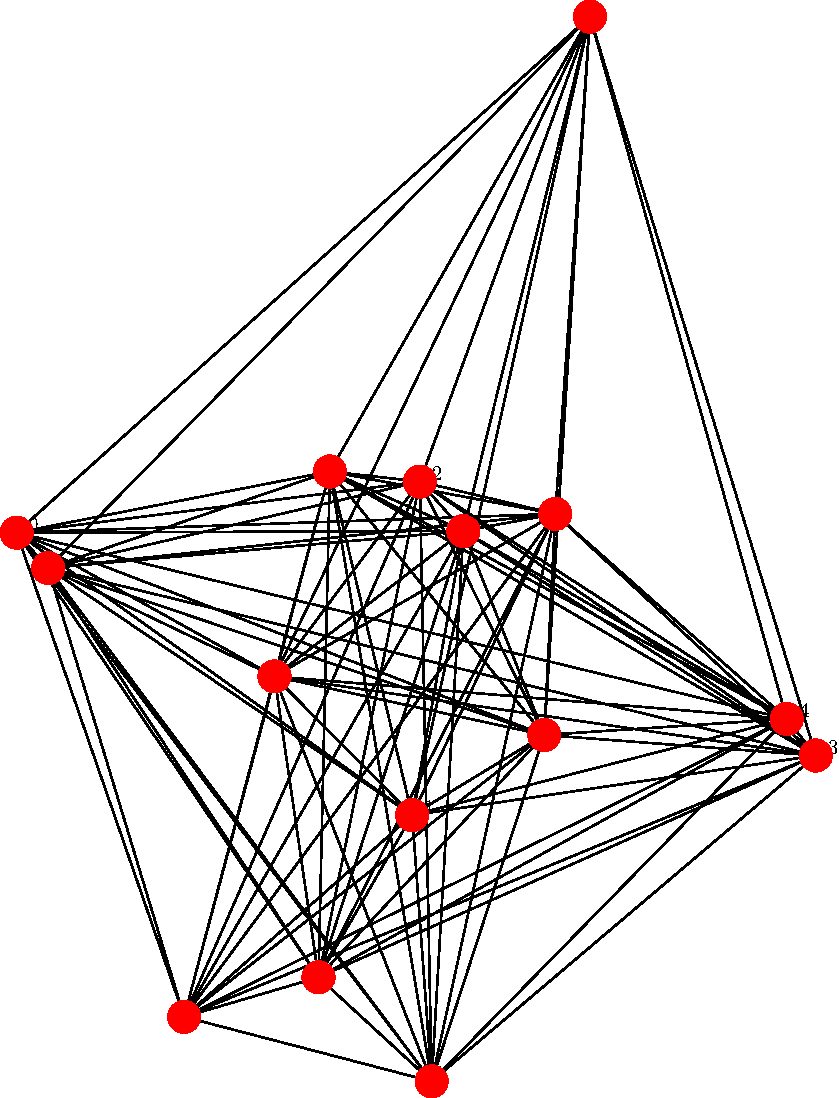
\includegraphics[scale=0.35]{smallgraph}
\]
\end{frame}

\begin{frame}
  \frametitle{Tropicalization of  $\frakX(F_2, \SL_3\bbC))$}
  The character variety $\frakX(F_2, \SL_3\bbC))$ is cut out by the
  polynomial
  {\tiny
  \[
    \begin{aligned}
      f= 9 &+ 3i - 6ab - 6cd - 6ef - 6gh + i^2 - abi - cdi - efi - ghi\\
      &+a^3 + c^3 + e^3 + g^3 + b^3 + d^3 + f^3 + h^3 - 3bhf - 3aeg - 3ceh\\
      &-3dfg + 3adh + 3bcg + 3acf + 3bde - abcdi + acfi + bdei + adhi\\
      &+bcgi + abcd + cdef + abgh + cdgh + abef + efgh + dh^2f + ceg^2\\
      &+ b^2dh + a^2cg + ad^2f + bc^2e + a^2hf + b^2eg + chf^2 + de^2g \\
      &+ b^2cf + a^2ed + ac^2h + bd^2g + d^2eh + c^2fg + aeh^2 + bfg^2 \\
      &+ be^2h + af^2g - 2bdf^2 - 2ace^2 - 2bch^2 - 2adg^2 + b^2d^2f \\
      &+ a^2c^2e + b^2c^2h + a^2d^2g - acd^2h - bc^2dg - a^2bcf - ab^2de \\
      &- ac^2df - bcd^2e - a^2bdh - ab^2cg - abd^3 - abc^3 - b^3cd - a^3cd
      \\
      &- bcdhf - acdeg - abceh - abdfg + a^2b^2cd + abc^2d^2
    \end{aligned}
  \]
  }

Its tropicalization $\Trop(\frakX(F_2,\SL_3\bbC))$ is the codimension 1
cones of the dual fan of the newton polytope $\rmN(f)$.
\end{frame}
\begin{frame}
  \frametitle{Big Graph}
  The edge graph of the Newton polytope is shown here
  $\frakX(F_2,\SL_3\bbC)$:
% big graph goes here
\[
  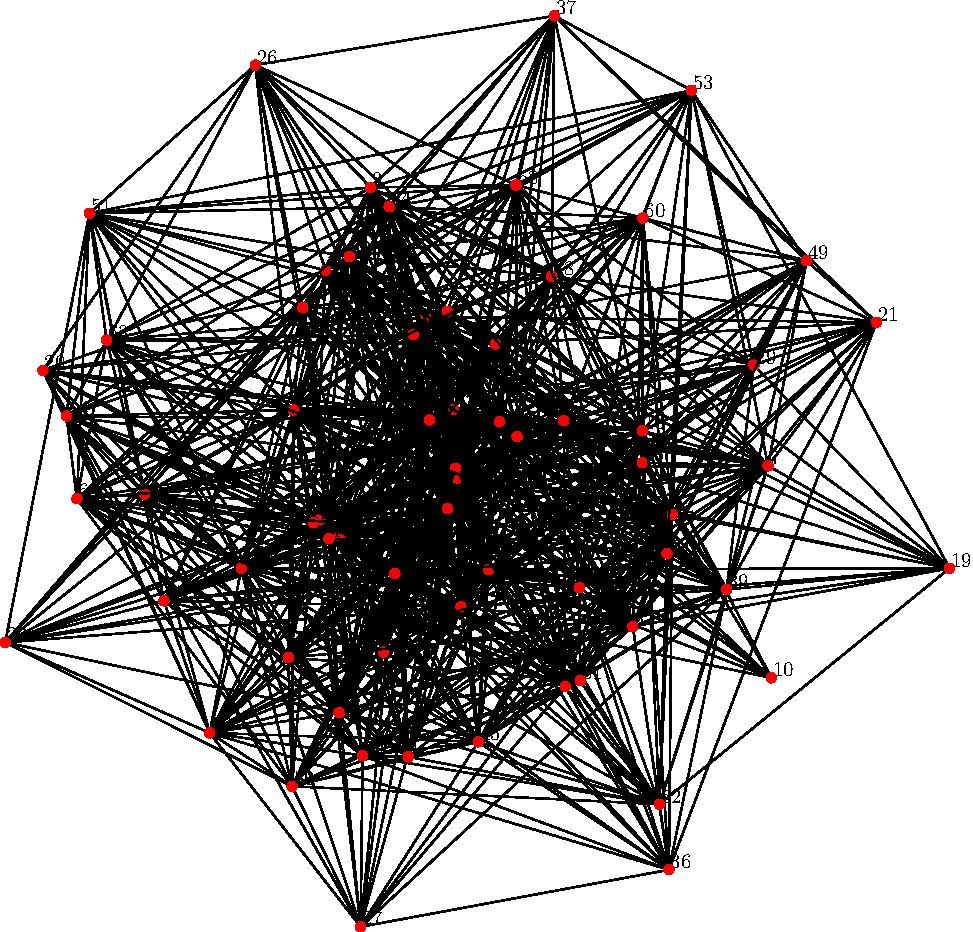
\includegraphics[scale=0.45]{biggraph}
\]
\end{frame}

%%% Local Variables:
%%% mode: latex
%%% TeX-master: "../MRC16-Trop-CharVars-Slides"
%%% End:
%
\begin{frame}
\frametitle{Generators}
Let $F_3=\langle A,B,C\rangle$.
$\bbC[\frakX(F_3,\PSL_2\bbC)]=\bbC[\frakX(F_3,\SL_2\bbC)]
^{\bbZ/2\bbZ\times\bbZ/2\bbZ\times\bbZ/2\bbZ}$ is
generated by:\\
\vspace{3mm} \textcolor{blue}{\emph{Type $\chi$}}
\begin{align*}
  \chi_A&\coloneq(\tr A)^2&\chi_B&\coloneq(\tr B)^2&\chi_C&\coloneq(\tr C)^2\\
  \chi_{AB}&\coloneq(\tr AB)^2&\chi_{AC}&\coloneq(\tr AC)^2 \\
  \chi_{BC}&\coloneq(\tr BC)^2&\chi_{ABC}&\coloneq(\tr ABC)^2
\end{align*}
\end{frame}

\begin{frame}
\frametitle{Generators cont.}
\textcolor{blue}{\emph{Type $\tau$}}
\begin{align*}
  \tau_{AB}&\coloneq\tr A\tr B\tr AB &\tau_{AC}&\coloneq\tr A\tr C\tr AC &\tau_{BC}&\coloneq\tr B\tr C\tr BC
\end{align*}
\pause
\textcolor{blue}{\emph{Type $\Lambda$}}
\begin{align*}
  \Lambda_A&\coloneq\tr B\tr C\tr AB\tr AC
  &\Lambda_B&\coloneq\tr A\tr C\tr AB\tr BC\\
  \Lambda_C&\coloneq\tr A\tr B\tr AC\tr BC
\end{align*}
\pause
\textcolor{red}{\emph{Lonely $\Delta$}}
\[
\Delta\coloneq \tr A\tr B\tr C\tr ABC
\]
\end{frame}

\begin{frame}
\frametitle{Generators cont.}
\textcolor{red}{\emph{Equally lonely $\Sigma$}}
\[
\Sigma\coloneq \tr AB\tr AC\tr BC
\]
\pause
\textcolor{blue}{\emph{Type $\Theta$}}
\begin{align*}
\Theta_A&\coloneq\tr A\tr BC\tr ABC&\Theta_B&\coloneq\tr B\tr AC\tr ABC \\
\Theta_C&\coloneq\tr C\tr AB\tr ABC
\end{align*}
\end{frame}

\begin{frame}
\frametitle{Relations}
Explicit example:
\[
\Sigma ^2=(\tr AB\tr AC\tr BC)^2=\chi_{AB}\chi_{AC}\chi_{BC}
\]
\end{frame}

\begin{frame}
\frametitle{(Binomial) Relations}
\begin{align*}
  \tau_{AB}^2&=\chi_A\chi_B\chi_{AB} &\tau_{AC}^2&=\chi_A\chi_C\chi_{AC}\\
  \tau_{BC}^2&=\chi_B\chi_C\chi_{BC}\\\\
  \Lambda_A^2&=\chi_B\chi_C\chi_{AB}\chi_{AC}
  &\Lambda_B^2&=\chi_A\chi_C\chi_{AB}\chi_{BC}\\
  \Lambda_C^2&=\chi_A\chi_B\chi_{AC}\chi_{BC}\\\\
  \Theta_A^2&=\chi_A\chi_{BC}\chi_{ABC}&\Theta_B^2&=\chi_B\chi_{AC}\chi_{ABC}\\
  \Theta_C^2&=\chi_C\chi_{AB}\chi_{ABC}\\\\
  \Sigma ^2&=\chi_{AB}\chi_{AC}\chi_{BC}&\Delta^2&=\chi_A\chi_B\chi_C\chi_{ABC}.
\end{align*}
\end{frame}

\begin{frame}
  \dots and finally the relation coming from $\frakX(F_3,\SL_2\bbC)$ can be
  written as
  \begin{align*}
    \begin{aligned}
      \chi_A&+\chi_B+\chi_C+\chi_{AB}+\chi_{AC}\\
      &+\chi_{BC}+\chi_{ABC}+\Sigma+\Delta
    \end{aligned}
    &=
      \begin{aligned}
        \tau_{AB}&+\tau_{AC}+\tau_{BC}\\&+\Theta_A+\Theta_B+\Theta_C+4.
      \end{aligned}
\end{align*}
\end{frame}

%%% Local Variables:
%%% mode: latex
%%% TeX-master: "../MRC16-Trop-CharVars-Slides"
%%% End:
%

%% Bibliography
% \begin{frame}[allowframebreaks]
%   \frametitle{References}
%   \cite{*}%
%   \bibliographystyle{plain}%
%   \bibliography{trop-charvar}%
% \end{frame}
\end{document}

%%% Local Variables:
%%% mode: latex
%%% TeX-master: t
%%% End:
